\section{Projektmanagement}\label{sec:projektmanagement}

Dieses Kapitel beschreibt die Planung und Organisation des Projekts.
Hierzu zählen das Organigramm in Abschnitt~\ref{subsec:Organigramm}, die Ablaufplanung in Form eines Gantt-Diagramms in~\ref{subsec:ablaufplan} und die Stakeholder- und Risikoanalyse in~\ref{subsec:Stakeholder-Risikoanalyse}.
Abschließend wird die Kosten- und Aufwandsplanung in Abschnitt~\ref{subsec:Kosten-Aufwandsplanung} und die Tools in~\ref{subsec:Tools} vorgestellt.

\subsection{Organigramm}\label{subsec:Organigramm}

\begin{figure}[H]
    \centering
    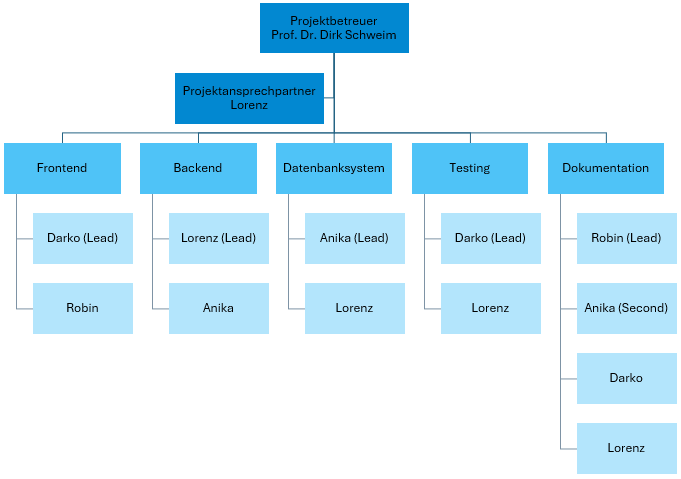
\includegraphics[width=0.8\textwidth]{organigramm}
    \caption{Organigramm}\label{fig:organigramm}
\end{figure}

Das Organigramm weist die Struktur und die Verantwortlichkeiten innerhalb des Projektteams auf.
Es gibt einen klaren Aufbau, der die verschiedenen Rollen und Zuständigkeiten verdeutlicht.

\begin{itemize}[itemsep=1em, leftmargin=*]
    \item \textbf{Projektbetreuer:}
    \begin{itemize}
        \item \textbf{Prof. Dr. Dirk Schweim:} Der Projektbetreuer steht an oberster Stelle und ist für die Betreuung des Projekts verantwortlich.
    \end{itemize}

    \item \textbf{Projektansprechpartner:}
    \begin{itemize}
        \item \textbf{Lorenz:} Der Projektansprechpartner steht direkt unter dem Projektbetreuer und ist für die Koordination und Kommunikation innerhalb des Teams als auch zum Projektbetreuer zuständig.
    \end{itemize}
    \newpage
    \item \textbf{Frontend:}
    \begin{itemize}
        \item \textbf{Hauptverantwortlich:} Darko
        \item \textbf{Vertretend:} Robin
        \item Die Frontend-Sparte ist für die Gestaltung und Implementierung der Benutzeroberfläche zuständig.
        Darko ist hauptverantwortlich für diese Abteilung, unterstützt von Robin.
    \end{itemize}

    \item \textbf{Backend:}
    \begin{itemize}
        \item \textbf{Hauptverantwortlich:} Lorenz
        \item \textbf{Vertretend:} Anika
        \item Das Backend kümmert sich um die serverseitige Logik und Datenverarbeitung.
        Lorenz ist der Hauptverantwortliche, wobei Anika unterstützend tätig ist.
    \end{itemize}

    \item \textbf{Datenbanksystem:}
    \begin{itemize}
        \item \textbf{Hauptverantwortlich:} Anika
        \item \textbf{Vertretend:} Lorenz
        \item Diese Sparte ist für die Verwaltung und Wartung der Datenbank zuständig.
        Anika hat die Hauptverantwortung, unterstützt von Lorenz.
    \end{itemize}

    \item \textbf{Testing:}
    \begin{itemize}
        \item \textbf{Verantwortlich:} Darko
        \item \textbf{Vertretend:} Lorenz
        \item Testing führt Tests durch, um die Qualität und Funktionalität der Plattform sicherzustellen.
        Darko verantwortet diesen Bereich, wobei die Aufgaben zu gleichen Teilen zwischen ihm und Lorenz aufgeteilt werden.
    \end{itemize}

    \item \textbf{Dokumentation:}
    \begin{itemize}
        \item \textbf{Hauptverantwortlich:} Robin
        \item \textbf{Vertretend verantwortlich:} Anika
        \item \textbf{Weitere Beteiligte:} Darko, Lorenz
        \item Die Dokumentation wird von allen im Projektteam erstellt und gepflegt.
        Robin ist hauptverantwortlich, Anika übernimmt eine vertretende Rolle, während auch Darko und Lorenz aktiv mitwirken.
    \end{itemize}
\end{itemize}


Diese Struktur weist eine klare Rollenverteilung und entsprechende Vertretung auf, die dem Projektteam ermöglicht, effizient und effektiv an Aufgaben zu arbeiten und ermöglicht eine bessere Zusammenarbeit.

\newpage

\subsection{Ablaufplanung}\label{subsec:ablaufplan}

Die Ablaufplanung dient dazu die zeitliche Abfolge und Dauer der einzelnen Teilaufgaben und Arbeitspakete übersichtlich zu veranschaulichen und so den Projektverlauf gezielt im Vorfeld zu planen.
Zur Visualisierung wurde ein Gantt-Diagramm mittels Microsoft Excel erstellt.
Die zeitliche Darstellung ist in Kalenderwochen skaliert.
Start des Semesters, wie auch des Moduls `Praxismodul I' ist gleichermaßen der 01.02.2024.
Frist der Abgabe des Projektberichts, wie auch der Präsentation ist der 19.06.2024, die Vorstellung der Ergebnisse findet am Folgetag statt.

Die einzelnen Arbeitspakete spiegeln den Projektstrukturplan aus Abschnitt~\ref{subsec:projektstrukturplan} zeitlich eingeordnet wider.
Die Teilaufgabe der Projektplanung beginnt zeitgleich des Modulstarts am 01.02.2024 mit der Anforderungsanalyse.
Mit Auswahl des zu bearbeitenden Themas und dessen Anforderungen innerhalb der ersten vier Wochen (inklusive Mock-Ups) erfolgt zudem die Projektplanung, das Projektmanagement und der Start der Dokumentation.
Nach Präsentation dieser Zwischenergebnisse am 21.03.2024 beginnt Ende März die technische Umsetzung anhand der Frontend- und Backend-Entwicklung, sowie Erstellung des Datenbanksystems.
Mit zwei Wochen Abstand startet auch die Teilaufgabe Integration und Deployment, welche ebenfalls Unit Testing und das Docker Deployment beinhaltet.
Alle Schritte sollen planmäßig mit dem Monatswechsel Juni abgeschlossen sein, um anhand dieses Standes und der Ergebnisse die Dokumentation rechtzeitig abzuschließen und die Abschlusspräsentation bis Mitte Juni zu erstellen.
Das Praxismodul I schließt mit erfolgreicher Präsentation am 20.06.2024 und Abgabe der Unterlagen am Vortag ab.

\begin{figure}[H]
    \centering
    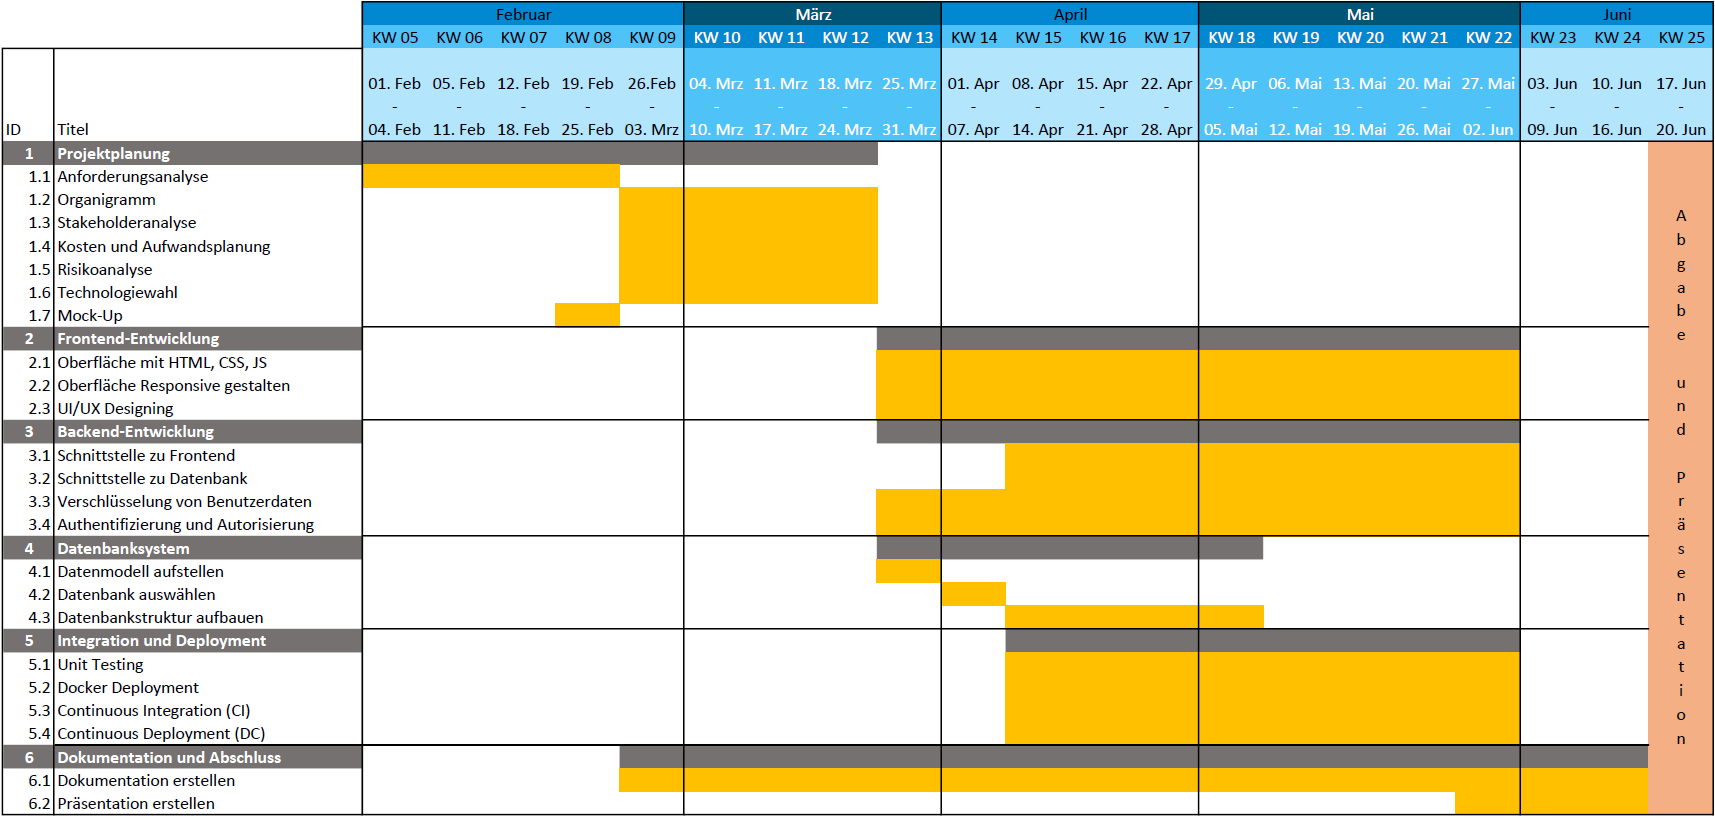
\includegraphics[width=1.0\textwidth]{gantt_chart_compact}
    \caption{Gantt-Diagramm}\label{fig:gantt-diagramm}
\end{figure}

\newpage

\subsection{Stakeholder- und Risikoanalyse}\label{subsec:Stakeholder-Risikoanalyse}
Im Folgenden wurde eine Analyse bezüglich der Stakeholder des Projektes erstellt.
Diese haben unterschiedliche Vorstellungen, Einstellungen und Ansichten zum Projekt.
Ergänzend wurde auch eine Risikoanalyse erstellt, welche zur Übersicht von eventuell eintretenden Problemen verhilft. \par
%WICHTIG: Nur nötig wenn die Grafik bei der fertigen Doku NICHT unter den oberen Absatz passt! LaTeX schiebt sonst die Grafik weit unpassend im Text runter. @lorack do u know a fix? -Anika
% Kommtenar Lorenz: Grafik kleiner machen indem du einen Wert vor \textwidth angibst (wie bspw. width=0.5\textwidth), ansosnten passt das mit \newpage, so habe ich das in BPM auch gemacht
%\Subsubsection{Stakeholderanalyse} \label{Stakeholderanalyse}

\begin{table}[h!]
    \centering
    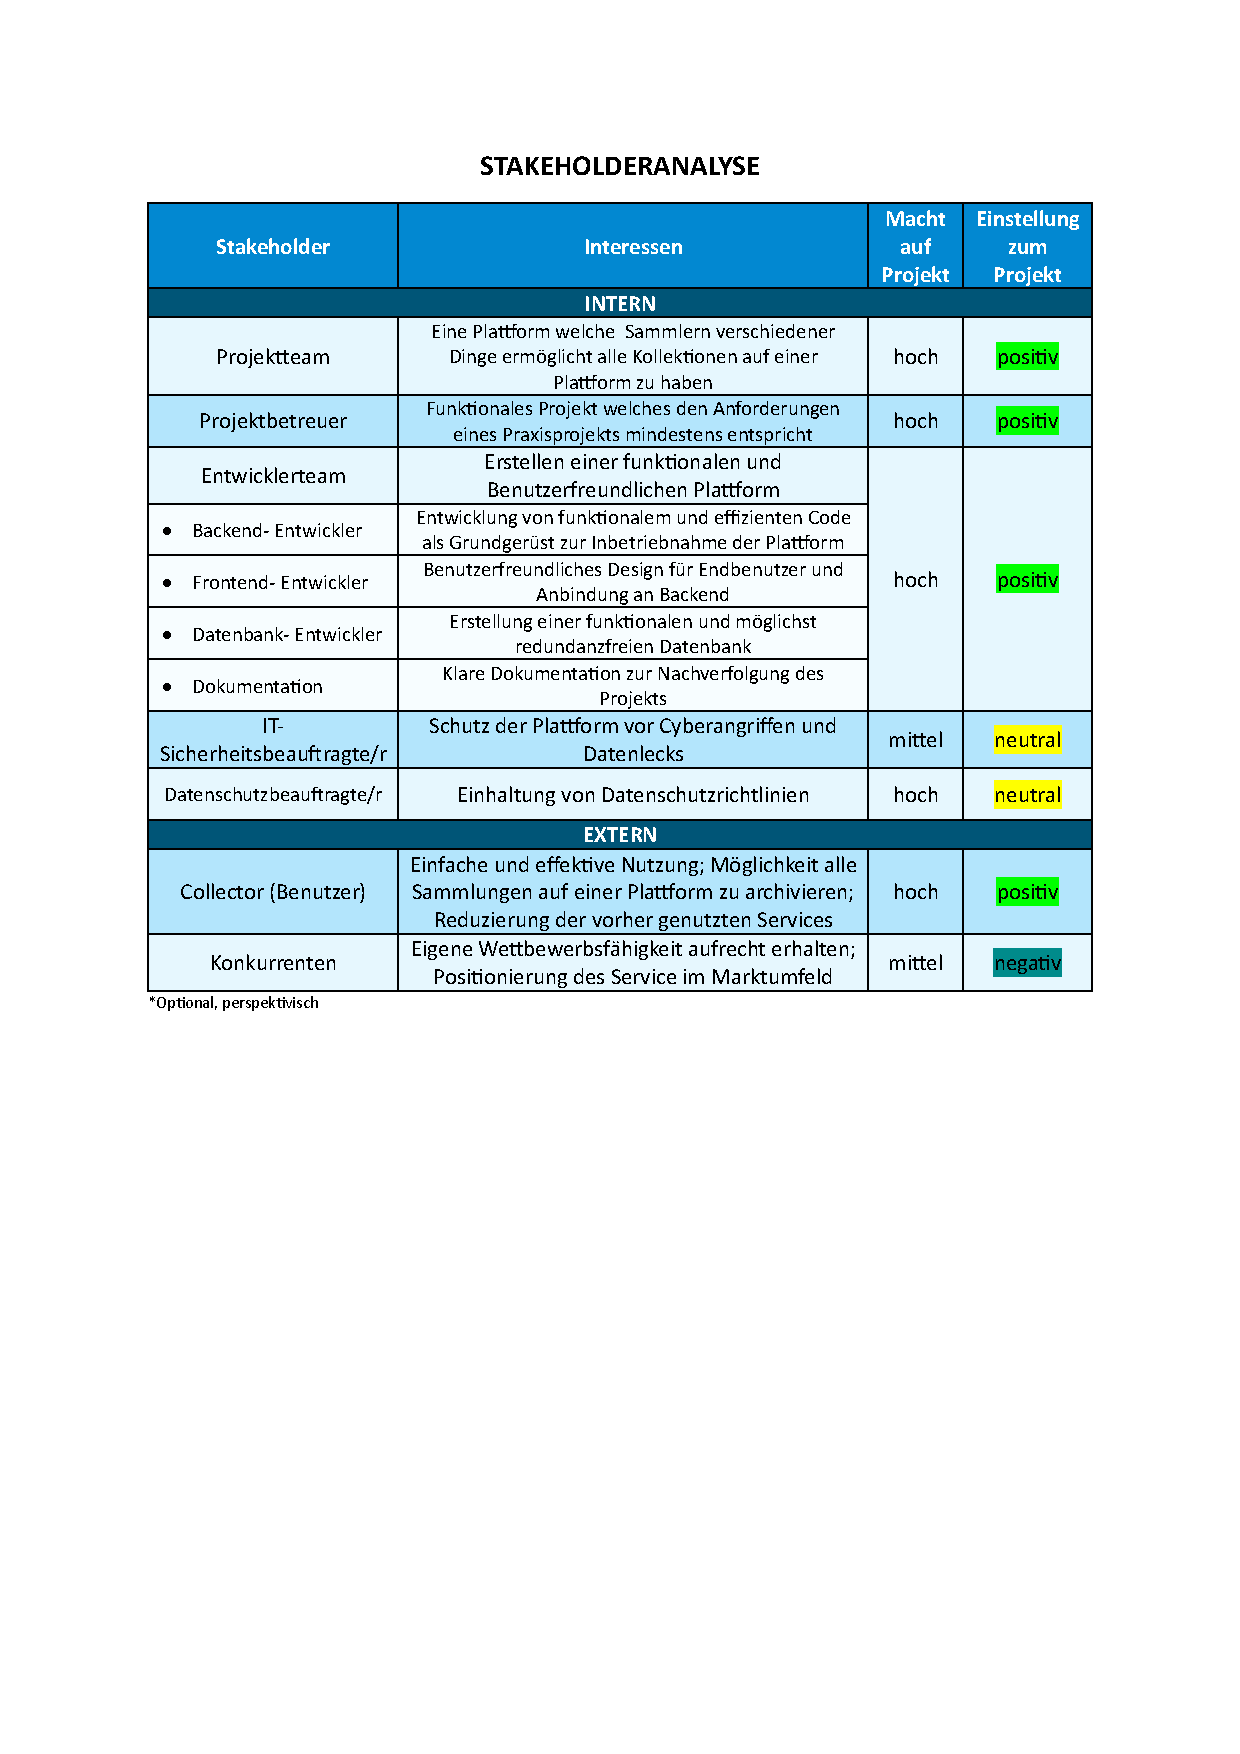
\includegraphics[width=0.9\textwidth, clip, trim=1cm 12.83cm 1cm 3cm]{PM_SH_RISK_ANALYSIS}
    \caption{Stakeholderanalyse}\label{tab:stakeholderanalyse}
\end{table}

Das Projektteam besteht aus Studierenden, die im Rahmen ihres Studiums die Plattform entwickeln.
Das Hauptziel des Teams ist analog zur Zieldefinition von Abschnitt~\ref{subsec:zieldefinition}.
Rückblickend auf die Motivation in Abschnitt~\ref{subsec:motivation} ist das Team positiv eingestellt. \par

Der Projektbetreuer hat ein starkes Interesse daran, dass das Projekt den Anforderungen eines praxisnahen Studienprojekts entspricht.
Sein Fokus liegt darauf, dass das Projekt nicht nur funktional, sondern auch innovativ und praxisnah ist.
Er hat erheblichen Einfluss auf den Projektverlauf und unterstützt das Team mit wertvollem Feedback und fachlicher Anleitung. \par

Das Entwicklerteam, welches aus dem Projektteam besteht, ist in mehrere spezialisierte Gruppen unterteilt, analog zum Organigramm in Abschnitt~\ref{subsec:Organigramm}.
Alle Entwicklergruppen haben parallel zum Projektteam-Stakeholder ein hohes Interesse am Projekterfolg und eine positive Einstellung zur Aufgabe.
Die einzelnen Interessen wurden zwecks persönlicher Lernerfolge nochmals aufgelistet. \par

Die Hauptnutzer der Plattform, die Sammelnden (Collector), stellen einen wesentlichen externen Stakeholder dar.
Ihr Interesse liegt in der einfachen und effektiven Nutzung der Plattform, die es ihnen ermöglicht, ihre Sammlungen zentral zu archivieren und die Nutzung mehrerer vorheriger Dienste zu reduzieren.
Ihre hohe Erwartung und positive Einstellung gegenüber der Plattform sind entscheidend für dessen Akzeptanz und Projekterfolg. \par

%\Subsubsection{Risikoanalyse} \label{Risikoanalyse}
%wichtig: Stake war in Präsens/Futur geschrieben, Risiko bewusst in Vergangenheitsform! >Discuss -Anika

\begin{table}[h!]
    \centering
    \includegraphics[page=2, width=0.9\textwidth, clip, trim=0.8cm 17.3cm 0.8cm 4cm]{PM_SH_RISK_ANALYSIS}
    \caption{Risikoanalyse}\label{tab:risikoanalyse}
\end{table}

Die Entwicklung einer universellen Sammlungsplattform wie Collectiqo wies verschiedene Risiken auf, die frühzeitig erkannt und gemindert wurden.
Eine gründliche Risikoanalyse ermöglichte es, potenzielle Herausforderungen zu identifizieren und geeignete Maßnahmen zu entwickeln, um den Projekterfolg sicherzustellen.

\begin{itemize}[itemsep=1em, leftmargin=*]
    \item \textbf{Technische Herausforderungen:} Ein bedeutendes Risiko bei der Entwicklung von Collectiqo lag in der technischen Komplexität des Projekts.
    Da das Projektteam bisher andere Anwendungsfelder bedient hatte, musste das vorhandene Wissen für das Projekt angeglichen und ergänzt werden.
    Um dieses Risiko zu minimieren, war es wichtig, eine gründliche technische Analyse vor Beginn des Projekts durchzuführen.
    Das Projektteam definierte klare und detaillierte Anforderungen und zog so verschiedene technische Lösungen in Betracht, um die Lernkurve entsprechend auf einem möglichen Level, aber dennoch herausfordernd für den eigenen Lernerfolg zu halten.

    \item \textbf{Kommunikationsprobleme:} Ein weiteres erhebliches Risiko bestand in möglichen Kommunikationsproblemen innerhalb des Projektteams.
    Da die Teammitglieder verschiedene Arbeitsweisen und Entwicklerstandards ihrer Unternehmen und eigener Erfahrung gewohnt sind, hätte es zu Verständnisproblemen kommen können, welche potentiell zu Verzögerungen, Qualitätsproblemen und einem schlechten Arbeitsklima geführt hätten.
    Um dieses Risiko zu bewältigen, war eine klare und regelmäßige Kommunikation entscheidend.
    Entgegenwirkend hielt das Team regelmäßige Meetings und verwendete YouTrack, um den Fortschritt zu verfolgen und sicherzustellen, dass alle Mitglieder auf dem gleichen Stand sind.

    \item \textbf{Verfügbarkeitsprobleme:} Ein weiteres Risiko bestand in möglichen Verfügbarkeitsproblemen, wie dem Ausfall von Services oder Hardware.
    Die Eintrittswahrscheinlichkeit wurde als mittel eingestuft, aber die Auswirkungen könnten den Projektfortschritt erheblich behindern.
    Um dieses Risiko zu minimieren, wurden Fall-Back-Alternativen und Lokalkopien erstellt, um die Arbeit auch bei Ausfällen fortsetzen zu können.
\end{itemize}


\subsection{Kosten- und Aufwandsplanung}\label{subsec:Kosten-Aufwandsplanung}
In der Kosten- und Aufwandsplanung soll die finanzielle, sowie zeitliche Ressourcenbindung für diese Projektarbeit näher betrachtet werden.
\begin{itemize}[itemsep=1em, leftmargin=*]
    \item\textbf{Kosten:} Die Projektmitglieder haben sich während der Planungsphase, basierend auf der Anforderungsanalyse, sowie dem Ziel und Thema des Projektes Gedanken über mögliche Kosten gemacht.
    Es wurde die Verwendung frei zugänglicher Software-Tools \& Education-Programme festgelegt.
    Abseits der eigenen zeitlichen Arbeitsleistung wird eine Kostenneutralität angestrebt.
    Das Budget für das Projekt wurde in Höhe von 0 € festgesetzt.

    \item\textbf{Aufwand:} Zur Abschätzung des zeitlichen Aufwandes wird auf das Modulhandbuch des Studiengangs zurückgegriffen, welches 15h Kontaktzeit und 110h Selbststudium jedes Studierenden für das Praxismodul I vorsieht.
    Die 15h der Kontaktzeit werden der initialen Einführungsveranstaltung des Moduls, den möglichen Coachingtermine mit dem Projektbetreuer, den regelmäßigen kurzen Team-Besprechungen und den zwei Präsentationsterminen zugeordnet.
    Aus Erfahrungswerten vergangener Projektarbeiten und Berücksichtigung der Abgabeleistungen werden von den 110h Selbststudium jeweils 10h für die Teilaufgabe der Projektplanung und 20h für die Ausfertigung der Dokumentation beziehungsweise Präsentation zugerechnet.
    Der größte zeitliche Anteil, die somit verbliebenen 80h fließen den technischen Teilaufgaben 2 (Frontend-Entwicklung) - 5 (Integration und Deployment), siehe Ablaufplanung - Abschnitt~\ref{subsec:ablaufplan}, über einen Zeitraum von Ende März bis Ende Mai zu.
    Da viele neue Tools bei diesem Projekt erstmalig für die Teammitglieder zum Einsatz kommen, ist davon auszugehen, dass ebenfalls eine intensivere Einarbeitung in diese notwendig ist.
    Rechnerisch ergibt sich in diesem zehnwöchigen Zeitraum ein Zeitaufwand von 8h pro Woche, wovon voraussichtlich jeweils 2h in die Einarbeitung der Tools entfallen.
    Die Projektarbeit wird vorwiegend an den Abenden beziehungsweise an Samstagen und Sonntagen aufgebracht.
\end{itemize}

\subsection{Tools}\label{subsec:Tools}
Dieser Abschnitt beschreibt die Anwendungen, die während der Planungsphase erarbeitet werden und für die Projektarbeit genutzt werden sollen.
Dreh- und Angelpunkt des Projektes als integrierte Entwicklungsumgebung ist WebStorm der Firma JetBrains angedacht.
GitHub dient als Ablageort des Remote Repositories, Versionsverwaltung und zwecks kollaborativen Arbeiten.
Als Aufgabenverwaltung wird das Produkt YouTrack, ebenfalls von JetBrains, eingesetzt.
Es soll eine Containerisierung mittels Docker einerseits für Front- und Backend, sowie anderseits für das Datenbanksystem genutzt werden.

Für das Frontend ist grundlegend klassisch HTML5 und CSS3 vorgesehen.
Hier soll zusätzlich das Framework Bootstrap mit der Webdesign- und Entwicklungsanwendung Bootstrap Studio zum Einsatz kommen.
Das Backend basiert auf Node.js.
Für Front- und Backend übergreifend kommt JavaScript zum Einsatz.
JavaScript ist plattformunabhängig und ermöglicht eine Integration des Webfrontends in verschiedenen Browsern und erleichterte die Implementierung von interaktiven Funktionen.

Das Datenbanksystem soll zwei Ansätze verfolgen.
Für strukturierte Daten - Nutzerdaten und für den Nutzer vorgefertigte Sammlungsvorlagen - ist ein relationales Datenbanksystem basierend auf MySQL angedacht.
Unstrukturierte Daten, hierzu zählen die für den Nutzer selbst erstellbaren Sammlungen, sollen in einem dokumentenorientierten NoSQL Datenbanksystem gespeichert werden.
Hier wird MongoDB angestrebt.

Die Projektdokumentation wird mithilfe von LaTeX erstellt.
Während des Moduls `Statistisches Forschungsprojekt' hatte sich das gemeinsame Arbeiten mittels Microsoft Word über OneDrive als sehr fehleranfällig herausgestellt.
Eine persistente Formatierung konnte nicht gewährleistet werden, ständig traten unerklärliche Veränderungen auf, die wiederholende zeitaufwendige Nachbesserung benötigten.
Microsoft Word und Excel dienen lediglich in kleinem Umfang der Zuarbeit anhand vereinzelter Tabellen und Abbildungen.
Die in Abschnitt~\ref{subsec:umfrage} erläuterten Umfrageergebnisse basieren auf Google Forms.
Für die Präsentation kommt weiterhin Microsoft PowerPoint zum Einsatz, welches über OneDrive der Hochschule geteilt wird.

Etwaige Rücksprachen und Coachings mit dem Projektbetreuer Herr Prof. Dr. Schweim werden in Präsenz oder mittels Videokonferenz basierend auf Zoom stattfinden.
Zoom wird gleichwohl auch für die regelmäßigen teaminternen Besprechungen Anwendung finden.
Microsoft Outlook dient hier der Kontaktaufnahme und für dessen Kalenderfunktion.

Die nachfolgende Abbildung~\ref{fig:uebersicht-tools} soll nochmals übersichtlich die soeben beschriebenen Tools für die Umsetzung des Projekts veranschaulichen.

\begin{figure}[H]
    \centering
    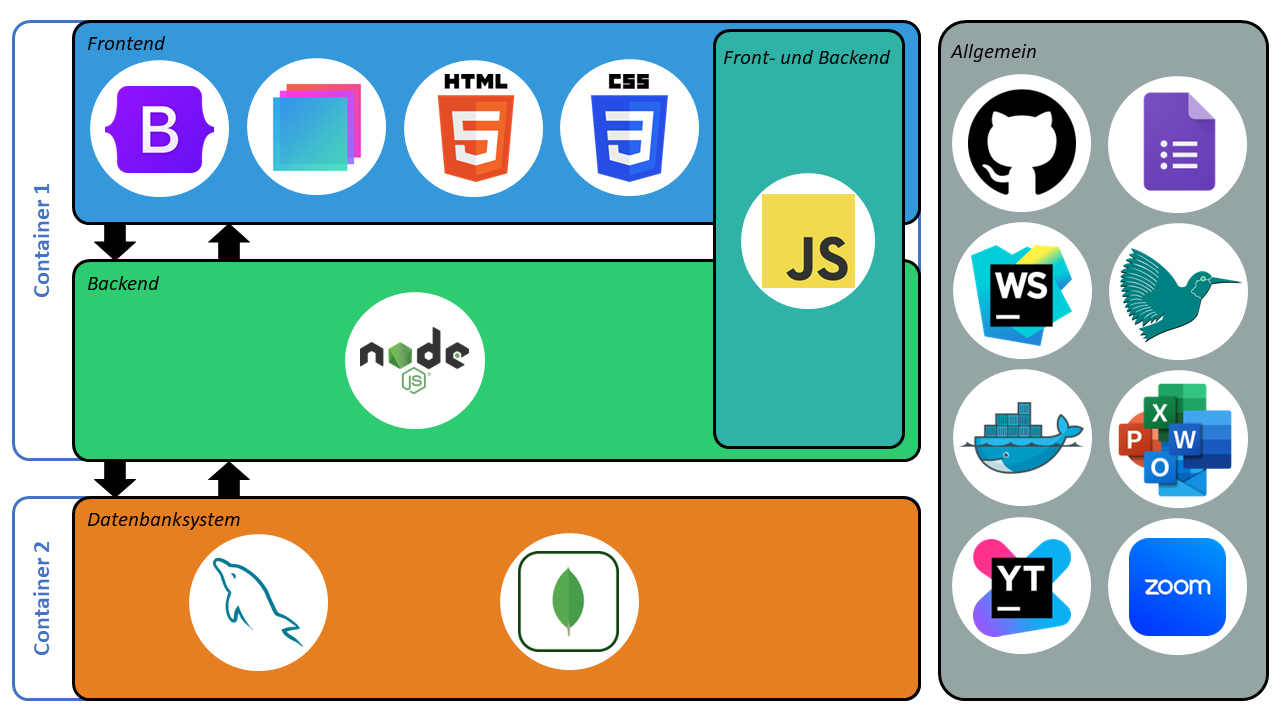
\includegraphics[width=1.0\textwidth]{tools_planning}
    \caption{Übersicht der Tools}\label{fig:uebersicht-tools}
\end{figure}
